\documentclass[conference]{IEEEtran}
\IEEEoverridecommandlockouts

\usepackage{cite}
\usepackage{amsmath,amssymb,amsfonts}
\usepackage{algorithmic}
\usepackage{graphicx}
\usepackage{textcomp}
\usepackage{xcolor}
\usepackage{url}

\def\BibTeX{{\rm B\kern-.05em{\sc i\kern-.025em b}\kern-.08em
    T\kern-.1667em\lower.7ex\hbox{E}\kern-.125emX}}

\begin{document}

\title{Introducing the Evolutionary Neuroplastic Agent (ENA): Dynamic Specialists for Non-Stationary Environments}

\author{
\IEEEauthorblockN{Blas Eugenio Vicco Zarate}
\IEEEauthorblockA{\textit{Independent Researcher}\\Valencia, Spain \\}
\IEEEauthorblockA{\texttt{blasvicco@gmail.com}}
}

\maketitle

Traditional Reinforcement Learning (RL) agents often struggle to adapt rapidly in non-stationary environments, suffering catastrophic forgetting when facing sudden physical shifts. Drawing inspiration from biological meta-learning and evolutionary diversity, this preliminary study introduces the Evolutionary Neuroplastic Agent (ENA). The ENA dynamically maintains an active population of multiple lightweight neural network policies (a ``pool of specialists") instead of a monolithic model. By continuously evaluating each specialist iteratively through defined \emph{Trust} and \emph{Plasticity} heuristics, the ENA autonomously triggers localized evolutionary search algorithms and substitutes specialists during environmental changes. We empirically evaluate two mechanisms for governing these shifts: a Quadratic Ratio formulation and a normalized Fuzzy-logic heuristic model. Evaluating this framework in a continuously shifting 1D CartPole domain transitioning across sequential gravities (Earth, Mars, Jupiter), we execute an online meta-learning testing protocol comparing frozen neural behaviors sequentially across those bodies tracking into a hidden fourth phase (Neptune). We demonstrate that the Fuzzy-logic framework manages inter-environment stability gaps smoothly. However, the study identifies critical limitations: the ENA exhibits massive standard-deviation dependencies on initial population states, confirming that robust adaptation within tightly constrained genetic boundaries remains highly vulnerable to initial parameter clustering. Our findings position the ENA as a promising proof-of-concept for dynamic Quality-Diversity adaptation, warranting further benchmarking against standard deep RL alternatives in complex domains.


\begin{IEEEkeywords}
Evolutionary Reinforcement Learning, Non-Stationary Environments, Plasticity, Quality-Diversity, Autonomous Adaptation
\end{IEEEkeywords}

\section{Introduction}

The widespread success of deep reinforcement learning (DRL) often hinges entirely on the presumption that the training environment distributions identically match the testing distributions. When operating in non-stationary environments—such as a robotic leg wearing down over time or shifting physics domains due to unpredictable conditions—canonical gradient-based methods such as Deep Q-Networks (DQN) notoriously suffer from \textit{catastrophic forgetting} \cite{mccloskey1989catastrophic}. When the parameters of an underlying transition function shift, the traditional DRL agent is forced to relearn its task from scratch, entirely unlearning the localized optimal policies of the previous state.

Biological organisms mitigate non-stationary environmental shifts through specialized plasticity, maintaining robust diverse memories or ``instincts" to rapidly switch behaviors when stimuli dramatically shift. Drawing inspiration from such mechanisms and from the burgeoning field of Quality-Diversity (QD) in Evolutionary Reinforcement Learning (ERL), we introduce the Evolutionary Neuroplastic Agent (ENA).

The ENA does not attempt to train a single generalized "master" neural network. Instead, it evolves a highly diverse \textit{population} of independent, lightweight neural network specialists. During run-time interacting with the environment, the ENA architecture mathematically abstracts its decision making through two critical metrics: \textit{Trust} (the evaluated confidence of the actively controlling specialist given the recent step rewards) and \textit{Plasticity} (the degree of exploration effort devoted across the "Hall of Fame" archive of other specialists). If the environment drifts into an unexplored physics regime, the ENA detects the performance drop, lowers trust in the failing specialist, scales its plasticity metric, and autonomously substitutes behavioral execution with another archived specialist whose genetic blueprint may better suit the new configuration. This substitution acts as an online meta-learning controller, selecting precisely which specialist will execute its frozen, pre-computed behaviors.

As a preliminary exploratory analysis, our work presents the following core contributions:
\begin{itemize}
    \item We detail the internal architecture of the ENA, emphasizing its continuous Trust decay system, Plasticity exploration search, and dynamic Hall of Fame entry gating strategy which utilizes z-score competitive protections to ensure genetic uniqueness within the archive.
    \item We rigorously evaluate the ENA using two isolated mathematical schemas for deriving Trust/Plasticity limits: a strict Quadratic Ratio bound, and a normalized Fuzzy-logic heuristic model.
    \item We demonstrate the ENA's performance across 10 independent experiments within a customized 1D kinematic CartPole toy domain featuring multi-gravity non-stationary constraints.
    \item We analyze the agent's variance limits connected directly to standard randomization population initializations, defining the statistical boundaries required for subsequent scaling.
\end{itemize}

This paper is structured systematically: Section II provides background on evolutionary reinforcement efforts including ERL and MAP-Elites. Section III defines the explicit methodology of ENA. Section IV breaks down our CartPole environment parameterizations. Section V and VI outline and discuss the experimental discoveries. 

\section{Related Work}

\subsection{Deep Reinforcement Learning \& Non-Stationary Environments}
Deep Reinforcement Learning (DRL) typically assumes that the underlying Markov Decision Process (MDP) remains stationary throughout training and deployment. When an environment transitions—such as shifting physics in robotics \cite{zhao2020sim} or varying task parameters—traditional methods like Deep Q-Networks (DQN) \cite{mnih2015human} suffer from catastrophic forgetting. Modifying weights to solve the newly presented environment invariably overwrites the synaptic memories associated with the previous tasks, leading to an inability to seamlessly generalize backwards once the environment shifts again.

\subsection{Evolutionary Reinforcement Learning (ERL)}
To bypass the limitations of single-agent gradient descent, Evolutionary Reinforcement Learning (ERL) merges population-based Evolutionary Algorithms (EA) with DRL gradient optimization \cite{khadka2018evolutionary}. ERL maintains a population of neural networks that share experiences and heavily map the parameter space, largely protecting the architecture from local minima. However, standard ERL often treats the population simply as a wide exploration mechanism for a single overarching actor. In contrast, ENA explicitly relies on the population as an ensemble of independent behavioral memories that can individually adapt to separate non-stationary sub-domains.

\subsection{Quality-Diversity and MAP-Elites}
Our methodology mathematically aligns with the emerging field of Quality-Diversity (QD) algorithms. Unlike traditional EAs that strive to discover a singular global optimum, QD algorithms like MAP-Elites \cite{mouret2015illuminating} explicitly seek to create an archive of diverse, high-performing behaviors. The work most parallel to our own is \textit{Intelligent Trial and Error} by Cully et al. \cite{cully2015robots}, which demonstrated that a robot with a broken leg could adapt in less than two minutes by searching a pre-computed MAP-Elites repertoire of alternative gaits. The Evolutionary Neuroplastic Agent (ENA) natively internalizes this paradigm; instead of depending on offline pre-computation, ENA autonomously regulates its diverse ``Hall of Fame" archive entirely online driven iteratively by its mathematical abstractions of Trust and Plasticity.

\section{Methodology}

The Evolutionary Neuroplastic Agent (ENA) architecture pivots completely on two interconnected heuristic values: Trust and Plasticity.

\subsection{Agent Initialization}
We maintain a population of $N=20$ independent specialists. Each individual specialist governs a lightweight Multi-Layer Perceptron comprising dense layers sized $(4, 2, |\mathcal{A}|)$ equipped with orthogonal initialization and ReLU activation. At the start of an episodic run, a single ``Active Specialist" is selected from the population to act upon the environment. The selection is dictated probabilistically during training by an exploration rate $\epsilon = 0.20$, and governed entirely by maximum archived \textit{Trust} rankings during test-time meta-adaptation.

\subsection{Trust Dynamics and Plasticity Formulations}
At the termination of an episode, the agent assesses the accumulated episodic reward $R \in [0, 500]$. Operating strictly as a non-gradient update, the agent mathematically penalizes or retains the active specialist by quantifying a failure signal, defined as the Trust Decay factor $D(R) \in [0.1, 1.0]$. The active specialist's unnormalized Trust score $T$ updates autoregressively:
\begin{equation}
    T_{t+1} = (1 - D(R_t)) T_t + D(R_t) R_t
\end{equation}
Consequently, an optimal decay rate $D=0.1$ gently smooths historical rewards, whereas a catastrophic failure rate $D=1.0$ instantly plunges the specialist's Trust exactly to the penalized $R_t$, ensuring it will be instantly abandoned in the subsequent sequence.

Simultaneously, the global \textit{Plasticity} variable defines the percentage of the remaining population that will be evaluated and mutated in response to the current episode's performance. Because exploration fundamentally mirrors trust failure, the defined Plasticity search volume $\mathcal{P}(R)$ is mathematically identical to the evaluated performance drop ($\mathcal{P}(R) \equiv D(R)$), linking exploration effort continuously to survival urgency. The shared heuristic algorithms evaluated for deriving $D(R)$ and $\mathcal{P}(R)$ are compared across two configurations:

\subsubsection{Fuzzy-logic Configuration (ENA-01)}
The fuzzy variant utilizes dynamic percentiles derived from a rolling reward history $H$. Let $P_{20}$ and $P_{90}$ denote the 20th and 90th percentiles of $H$.
\begin{equation}
    D_{fuzzy}(R) =
    \begin{cases}
        0.1 & \text{if } R \ge P_{90} \\
        1.0 & \text{if } R \le P_{20} \\
        1.0 - 0.9 \left( \frac{R - P_{20}}{P_{90} - P_{20} + 10^{-8}} \right) & \text{otherwise}
    \end{cases}
\end{equation}

\begin{figure}[htbp]
\centerline{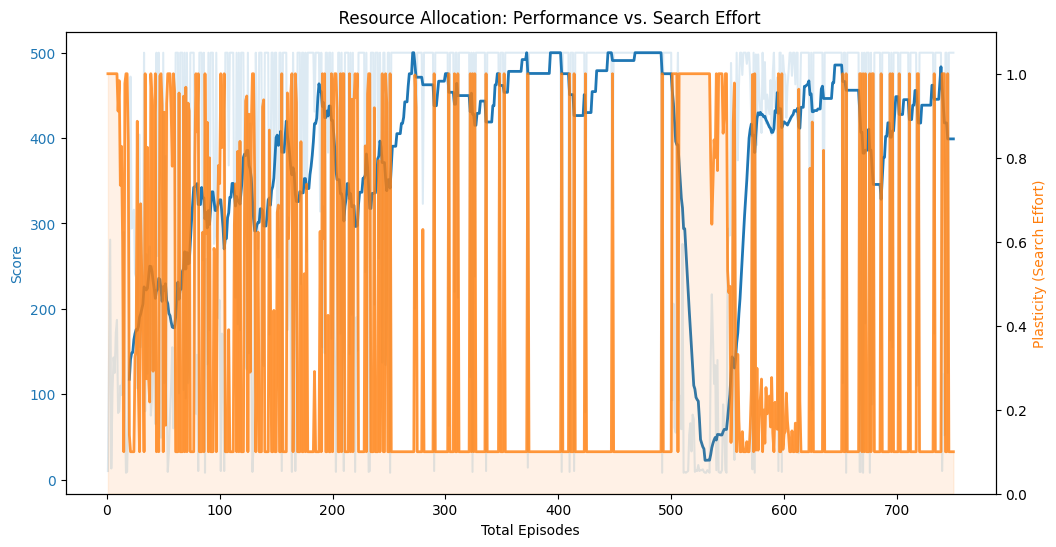
\includegraphics[width=\linewidth]{images/plasticity_ena_01.png}}
\caption{Plasticity search effort and algorithmic response mapped against the episode score average for the Fuzzy-Logic ENA-01 configuration. Spikes indicate triggered evolutionary search due to trust failure.}
\label{fig:plasticity}
\end{figure}

\subsubsection{Quadratic Ratio Configuration (ENA-02)}
The strictly mathematical variant derives loss squarely against the absolute extrema observed, clipping and penalizing failures quadratically:
\begin{equation}
    D_{quad}(R) = \min \left(1.0, \max \left(0.1, \left( \frac{R_{max} - R}{R_{max} - R_{min} + 10^{-8}} \right)^2 \right)\right)
\end{equation}

\subsection{Competitive Hall of Fame (Specialist Archive)}
To protect highly-skilled specialists, ENA regulates a structurally constrained Hall of Fame archive capped at a maximum of $K=5$ distinct specialists. This deliberate bottleneck enforces extreme genetic selectivity, ensuring only the most versatile behavioral archetypes survive long-term. An active specialist only earns induction if its performance achieves a statistically significant Z-score relative to the active population: $Z = (T_{old} - \mu_{T}) / (\sigma_{T} + 10^{-8})$. We dynamically lower induction barriers during periods of high environmental flux (high Plasticity) according to the threshold boundary: $Z_{req} = 1.5 \times (1.0 - (\text{Plasticity} \times 0.5))$.

To prevent early-discovered specialists from permanently dominating the archive, we apply an ``age-of-discovery'' memory decay mechanism. At every evolutionary check, the recorded induction Z-score of each archived specialist decays multiplicatively: $Z_{stored} \leftarrow Z_{stored} \times 0.995$. This ensures that archaic specialists gradually become vulnerable to replacement by stronger current-generation candidates, implementing an active form of bounded forgetting that prevents archive stagnation.

Once successfully evaluated for induction, a genetic similarity constraint computationally measures the flattened cosine similarity of the neural weights between the candidate and existing archive members $S_{cos\_sim} = \frac{W_a \cdot W_b}{\|W_a\|\|W_b\| + 10^{-8}}$. If two specialists are effectively identical genetically ($S_{cos\_sim} \ge 0.95$), the newer iteration battles its twin specifically based entirely on comparative Z-scores. This niche protection mechanism preserves the distinct uniqueness of isolated physics environments inside the archive without replacing structurally unique behaviors.

\subsection{Evolutionary Search Steps}
If the computed $D(R)$ rises above $0.1$, indicating the baseline trust is failing within a non-stationary physics shift, an evolutionary step is forcefully triggered. A fixed generational strategy budget governs how the next population is constructed: the top 20\% of specialists by Trust score are preserved as elites; 30\% of the new generation is produced by mutating elite parents via $\mathcal{N}(0, 0.1)$ Gaussian noise applied to a sparse 1\% of synaptic connections; a further 30\% is produced by crossover between randomly paired elites, applying a 50\% uniform random binary weight-mask per synaptic layer; and the remaining 20\% are entirely fresh randomly-initialized individuals injected to protect population-level genetic diversity. Additionally, when a catastrophic failure is detected, the Trust scores of all non-elite specialists are not reset to zero but are instead re-anchored to the dynamic historical mean $\mu_{history} = \text{mean}(H)$, preserving relative competitive rankings while preventing stale specialists from falsely dominating.

\section{Experimental Setup}

To evaluate the ENA's non-stationary domain adaptation, we executed an intensive multi-phase analysis using a modernized variant of the classic \texttt{CartPole-v1} environment parameterized entirely through modified kinematics.

\subsection{Environmental Domains}
Rather than shifting observation states, our domain randomization modifies the fundamental gravitational kinematics acting upon the pole mass. We simulated the physical traits of celestial environments:
\begin{itemize}
    \item \textbf{Training Sequence:} Earth ($g = 9.8 \text{ m/s}^2$), Mars ($g = 3.7 \text{ m/s}^2$), and Jupiter ($g = 24.8 \text{ m/s}^2$).
    \item \textbf{Testing Sequence:} We evaluate the frozen multi-policy archive progressively through the familiar training bodies (Earth, Mars, Jupiter) to test structural retention, immediately followed by a hidden fourth testing world: Neptune ($g = 11.15 \text{ m/s}^2$), strictly withheld from all prior evolutionary searches.
\end{itemize}

\subsection{Evaluation Parameters}
We quantified the evolutionary behavior over 10 randomized and independent experiments. Each instance constrained training to an upper bound of 250 episodes per environment phase. Following training, the evolutionary update matrices (\textit{Plasticity}) and gradients were frozen while executing the agents over the testing regime to measure test-time domain generalization dictated entirely by the online meta-learning specialist archive selector acting over the frozen behaviors.

\subsection{Test Configurations}
Three distinct computational profiles were assessed to determine optimal Trust/Plasticity behavior:
\begin{itemize}
    \item \textbf{ENA-01:} Employed the percentile-based Fuzzy-logic heuristic for calculating Trust decay and Plasticity metrics across all phases.
    \item \textbf{ENA-02:} Functional Baseline. Employed the purely deterministic Quadratic Ratio formula across all phases, acting as a standard mathematical archive-selector comparison against the fuzzy heuristic.
    \item \textbf{ENA-03:} Utilized the trained Hall of Fame archive established by the Fuzzy-logic search mechanisms (identical to ENA-01 during training), but aggressively overrode Trust calculations during the testing phase utilizing the continuous Quadratic decay heuristic.
\end{itemize}

\section{Results and Performance Analysis}

Operating across the hidden Neptune physics constraints, the accumulated testing phase results reveal the distinct operational trends afforded by the diverse ENA configuration modalities. Performance was quantified by averaging reliability thresholds across all 10 experimental runs.

\subsection{Online Testing Reliability \& Stability Gaps}
Across the four-world Testing sequence, varying success metrics illuminated explicit architectural gaps between the models. \textbf{ENA-03} achieved a marginally higher overarching Mean Reliability ($85.18\%$) compared to the pure Fuzzy-logic \textbf{ENA-01} ($84.91\%$) and Quadratic \textbf{ENA-02} baseline ($76.46\%$).

However, maximum absolute reliability does not translate to maximum \textit{adaptive stability}. To quantify shift-resilience, we calculated the ``Stability Gap"—defined as the mean score delta between the 20 episodes strictly preceding a gravitational shift and the 20 episodes immediately following it ($\Delta = \text{Score}_{pre} - \text{Score}_{post}$). An optimal transition gap approaches $0$, indicating the agent seamlessly retained baseline mastery without needing multi-episode transition recoveries.

Here, \textbf{ENA-01} out-scaled its counterparts. Operating purely on fuzzy mechanics, ENA-01 yielded a mathematical Stability Gap of only $-2.13$ ($\sigma = 4.66$). Because the second environment (Mars) physically allows higher survival intervals than Earth, negative values indicate expected score increases. ENA-01 transitioned smoothly with minimal variance. In contrast, ENA-03 demonstrated an inter-environment gap of $-20.89$ ($\sigma = 49.85$). This extremely high standard deviation on ENA-03 implies that aggressive quadratic trust-decay caused volatile behavior precisely during the transition boundary, whereas the fuzzy-logic configuration smoothed the evolutionary migration.

\begin{table}[htbp]
\caption{Testing Performance Across 10 Experiments (Without Significance Scaling)}
\begin{center}
\begin{tabular}{|c|c|c|c|c|}
\hline
\textbf{Configuration} & \textbf{Reliability} & \textbf{Rel. Std ($\sigma$)} & \textbf{Stability Gap} & \textbf{Gap Std ($\sigma$)} \\
\hline
ENA-01 & 84.91\% & 28.87\% & -2.13 & 4.66 \\
ENA-02 & 76.46\% & 21.14\% & -14.15 & 39.13 \\
ENA-03 & 85.18\% & 28.02\% & -20.89 & 49.85 \\
\hline
\end{tabular}
\label{tab:metrics}
\end{center}
\end{table}

\begin{figure}[htbp]
\centerline{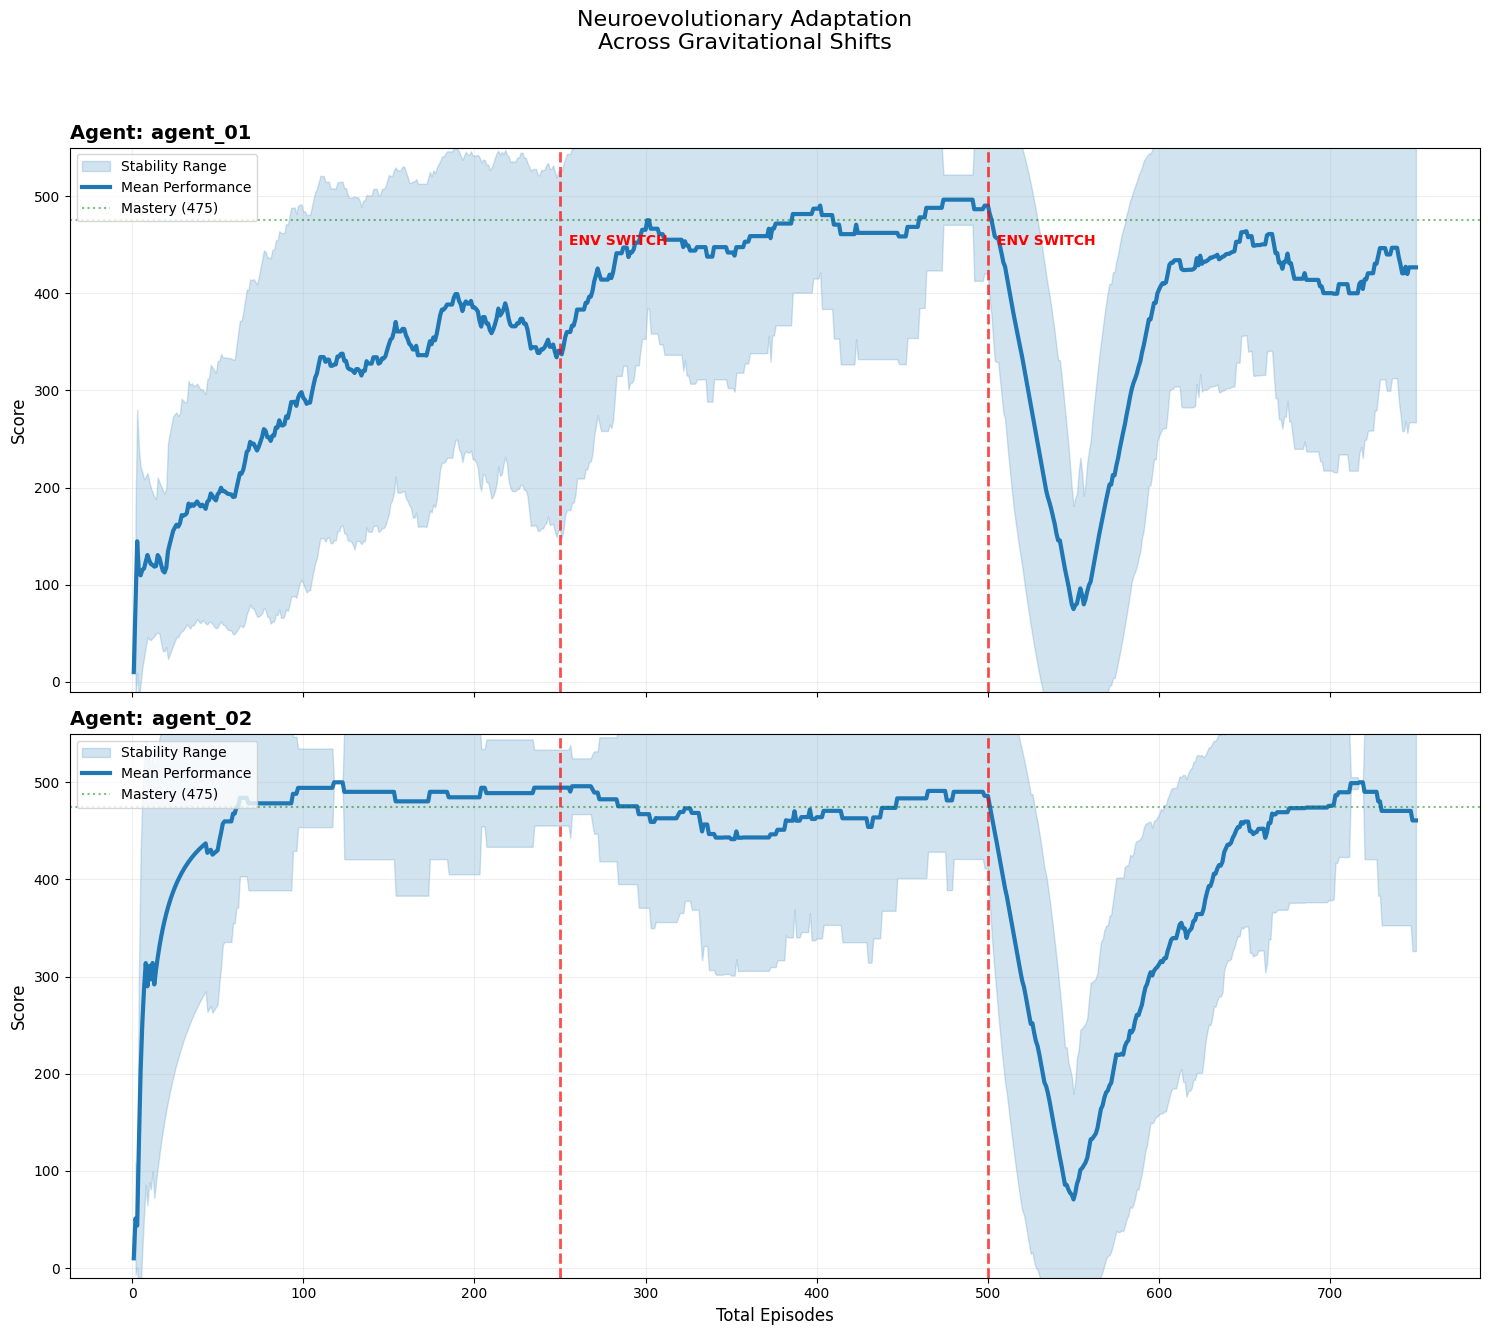
\includegraphics[width=\linewidth]{images/training_exp_01.png}}
\caption{Academic performance tracking the stability gap and deviation matrices over varying gravitational domain shifts (red markers).}
\label{fig:academic}
\end{figure}

\begin{figure}[htbp]
\centerline{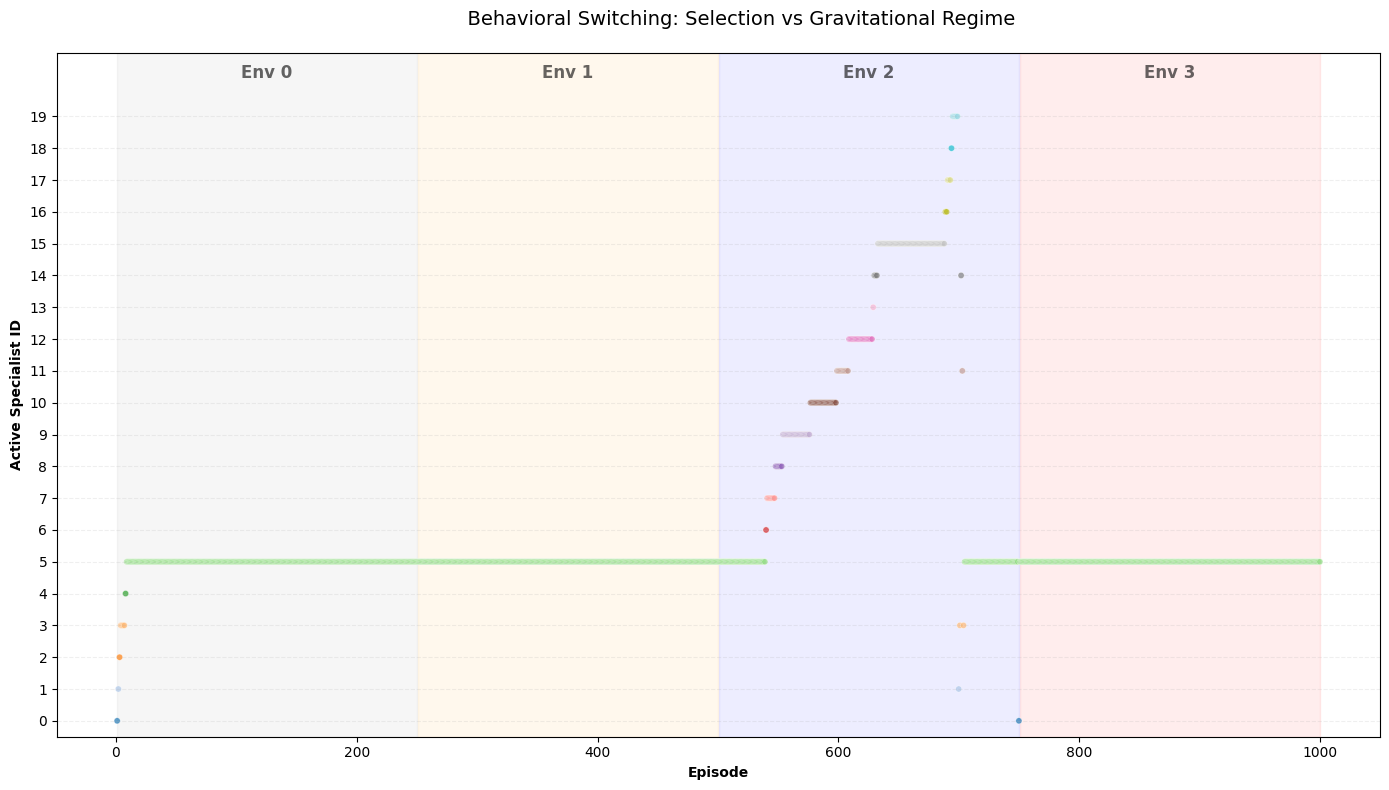
\includegraphics[width=\linewidth]{images/test_active_specialist_ena_01.png}}
\caption{Active Specialist behavioral switching matrix, directly plotting the specific Hall of Fame identity assumed sequence-to-sequence as the overarching gravitational parameters shift.}
\label{fig:specialist}
\end{figure}

\subsection{Initialization Variance and Evolutionary Constraints}
While ENA-01 demonstrated strong macroscopic testing generalizations, the 10 independent experiments strictly revealed profound macroscopic variance vulnerabilities. It is important to explicitly state that the vast standard deviations observed across merely 10 independent runs mathematically prohibit assigning strict statistical significance to the absolute superiority of ENA-01 over the baselines without future intensive t-test scaling; we analyze the outcomes here strictly as observed empirical trends.

Despite averaging an impressive $84.91\%$ reliability, ENA-01 reported an immense testing Standard Deviation ($\sigma = 28.87\%$). Analyzing individual experimental extrema revealed maximum testing mastery reaching a near-perfect $99.60\%$, abruptly contrasted by minimum catastrophic testing failures resolving at $0.80\%$ reliability.

This suggests that beneath constraints of a tiny localized computational window (population size $N=20$, absolute duration bound $250$ episodes), the Evolutionary Neuroplastic Agent remains highly reliant on the initial randomization matrices (often termed ``lucky" initializations). The $0.80\%$ test performance minimum highlights a potential mathematical vulnerability (pending future strict seed-control isolation studies): if initialized poorly, the limited ENA population narrowly overfits to its sequential training zones. Unable to properly illuminate the evolutionary space, the resultant Hall of Fame is physically unequipped to respond to hidden structural regimes like Neptune, resulting theoretically in localized test-time performance collapse.

\begin{figure}[htbp]
\centerline{
\includegraphics[width=\linewidth]{images/reliability_box.png}}
\caption{Box plot delineating the distribution spread of test-time Reliability across 10 randomized population initializations. The presence of single percentage extrema confirms extreme algorithmic vulnerability to early-generation population clustering.}
\label{fig:reliability_box}
\end{figure}

\begin{figure}[htbp]
\centerline{
\includegraphics[width=\linewidth]{images/stability_bar.png}}
\caption{Bar chart displaying Mean Stability Gaps $\pm 1\sigma$. The ENA-01 (fuzzy bounds) statistically mitigates non-stationary adaptation losses radically more efficiently than ENA-03.}
\label{fig:stability_bar}
\end{figure}

\section{Conclusion and Future Work}

We introduced and evaluated the Evolutionary Neuroplastic Agent (ENA), an algorithmic framework fundamentally designed to combat catastrophic interference over shifting environments by maintaining a highly responsive, continuously updated archive of sub-specialists governed competitively through heuristic \textit{Trust} and \textit{Plasticity} limits. Extensive evaluation across changing physical gravities established that deploying Fuzzy-logic metric derivations substantially minimized the observed Stability Gap during domain adjustments (down to $-2.13$) when juxtaposed against deterministic quadratic ratio limits. The mechanism allows an algorithmic bridging between pure Quality-Diversity maps and direct continuous reinforcement agents.

Crucially, experimentation unveiled the direct limitations dictated by initialization variance on populations. Constraining learning vectors to limited search spaces can produce unpredictable isolated performance degradation (represented by instances diving toward $0.80\%$ capability), heavily supporting the hypothesis that robust adaptation demands substantial initialized genetic diversity.

Future work will expand the analysis beyond the preliminary 1D kinematic CartPole benchmark by scaling generation counts and population pools sequentially into deeper continuous domains. By mathematically eroding the initialization bottleneck, we plan to directly benchmark ENA's overarching rapid-learning mechanisms continuously against established baseline DRL frameworks (such as PPO or Deep Q-Networks) to validate absolute operational supremacy.

\section*{Code Availability}

To support reproducibility and open science, the full implementation of the Evolutionary Neuroplastic Agent is publicly available. The repository contains the complete experimental codebase, LaTeX source for this paper, and helper scripts for aggregating and visualizing results.

\begin{itemize}
    \item \textbf{GitHub Repository:} \url{https://github.com/blasvicco/ena}
    \item \textbf{Interactive Notebook (Google Colab):} \url{https://colab.research.google.com/drive/1n3wp9BR7GoUn0Ym-DSwGNGdwIwhafQqY?usp=drive_link}
\end{itemize}

The Colab notebook provides a self-contained, zero-setup environment in which all 10 independent experiments can be reproduced directly in a browser without any local installation.


\bibliographystyle{IEEEtran}
\bibliography{references}

\end{document}
